% DO NOT COMPILE THIS FILE DIRECTLY!
% This is included by the other .tex files.

\begin{frame}[t,plain]
  \titlepage
\end{frame}


\begin{frame}
\frametitle{Outline} % Table of contents slide, comment this block out to remove it
  \tableofcontents % Throughout your presentation, if you choose to use \section{} and \subsection{} commands, these will automatically be printed on this slide as an overview of your presentation
\end{frame}

%----------------------------------------------------------------------------------------
% PRESENTATION SLIDES
%----------------------------------------------------------------------------------------

%------------------------------------------------
\section{Introduction} % Sections can be created in order to organize your presentation into discrete blocks, all sections and subsections are automatically printed in the table of contents as an overview of the talk
%------------------------------------------------

%\subsection{Introduction} % A subsection can be created just before a set of slides with a common theme to further break down your presentation into chunks

\begin{frame}
\frametitle{Introduction}
  91Dict is a dictionary application developed by
  \begin{enumerate}[1.]
    \item C programming language
    \item Data Structure Btree 
    \item Gtk+ 3.0 library for graphical user interface (GUI)
  \end{enumerate}
\end{frame}

%------------------------------------------------
\section{Overview and Usage}

\begin{frame}
\frametitle{Overview and Usage}
\begin{itemize}
  \item 3 different dictionaries
  \begin{enumerate}[1.]
    \item FOLDOC
    \item English Vietnamese Dictionary
    \item Vietnamese English Dictionary
  \end{enumerate}
  \item Program feature
  \begin{enumerate}[1.]
    \item Add word
    \item Edit word
    \item Delete word
    \item Bookmark
    \item Suggests word
    \item Search Entry Autocomplete (by History)
  \end{enumerate}
\end{itemize}
\end{frame}

\begin{frame}
  \frametitle{Overview and Usage}
  \centering{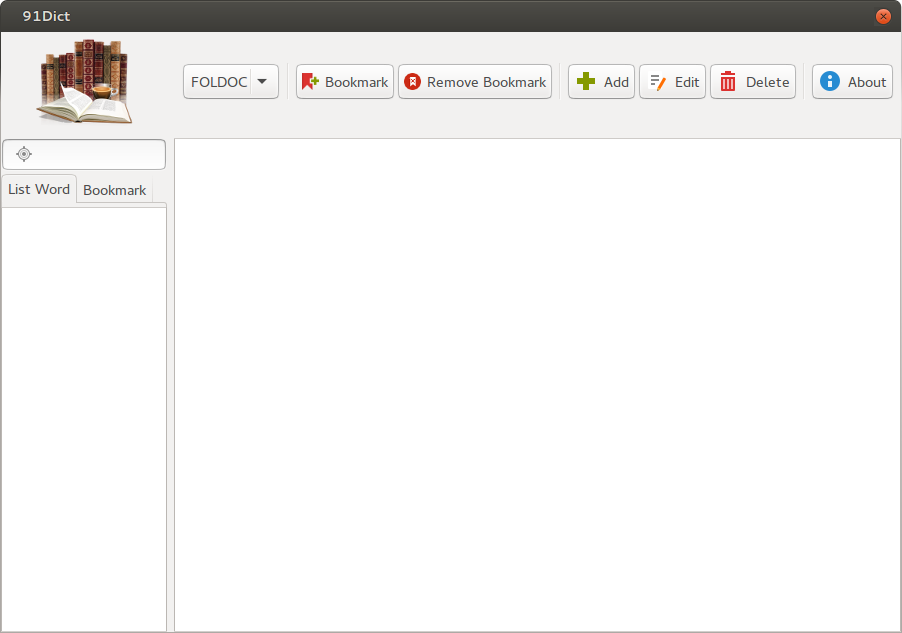
\includegraphics[width=0.9\textwidth]{img.png}};
\end{frame}

\subsection{Shortcut}
\begin{frame}
  \frametitle{Shortcut}
  \begin{itemize}
    \item $`ctrl + n`$       : Add new word
    \item $`ctrl + e`$     : Edit current search word or selected word  
    \item $`shift + delete`$ :  Delete current search word or selected word
    \item $`ctrl + d`$    : bookmark word  
    \item $`ctrl + delete`$ : delete bookmark selected word on bookmark 
  \end{itemize}
\end{frame}

%------------------------------------------------
\section{Data structure design}

\begin{frame}
\frametitle{Data structure design}
91Dict use Btree for data structure for storage data
\begin{itemize}
  \item Dictionary (key: word, value: meaning)
  \item Soundex (Key: Soundex String, value: list of words has same soundex string \
separated by semi-colon $;$)
  \item Bookmark (Key: word, value : 1)
  \item History for search entry autocomplete (Key: word, value : 1)
\end{itemize}
\end{frame}

%------------------------------------------------

%------------------------------------------------
\section{Data source and References}
\begin{frame}
\frametitle{Data source and References}
\begin{itemize}
  \item Btree $http://www.hydrus.org.uk/doc/bt/html/$
  \item GTK+ 3.0 $http://www.gtk.org/$
  \item Glade help for design $https://glade.gnome.org/$
  \item 91Dict Source Code $https://github.com/91ICT/91Dict$
\end{itemize}
\end{frame}
%------------------------------------------------

\begin{frame}
\Huge{\centerline{The End}}
\end{frame}
